
\part[State of the Art]{Using applications at the Edge: a state of the art}
\label{p:soa}

\epigraph{We got tactical smart missiles, phased plasma pulse rifles, RPGs, we got sonic electronic ball breakers! We got nukes, we got knives, sharp sticks...}{Private Hudson, Aliens}


\begin{comment}
* Using applications at the Edge: a state of the art - 45p
** Developing an application for the Edge - 20p
** Managing the Edge infrastructure - 20p
** Using Cloud Applications at the Edge - 5p
\end{comment}

In this part, we will compare academic and industry approaches
to put an application at the Edge.
%
We have seen in the previous part (\autoref{sec:why-no}) how
approaches to deal with the collaborations to provide a single
coherent system are not satisfying.
%
Now, we will investigate how other approaches can be made without
necessarily having to deal with the collaborations, by pushing
applications to the Edge in different manners.
%based on the requirements we defined in~\autoref{sec:principles}.

The goal of this part is mainly to study interesting solutions in the
literature to first, obviously, avoid reinventing the wheel.
%
This will be ensured by the comparison of our requirements to these
approaches; if they fit my requirements, it is not necessary to make
it from scratch.
%
Second, even if some requirements are not enforced, parts of the
approaches can be interesting to build my own approach, and thus
answer the questions raised.
%
Finally, it can be useful to give insights of functioning ideas that
do not fit our requirements to be able to question them.


Because I wanted my solution to be generic to a lot of Cloud
applications, there is a broad spectrum of approaches that can be of
interest to us.
%
As a smaller goal, I tried to focus on the most interesting approaches
regarding our requirements and/or the representativity of the solution
for each section.

First, I present in~\autoref{chap:comparison} the comparison points
based on the requirements we defined in~\autoref{sec:principles}.
%

%
\autoref{chap:soa-edge-infra} presents ways to manage the Edge
infrastructure so we can deploy applications on it.
%
In particular, \autoref{chap:soa-SM} presents service meshes for the
Cloud to explore the possibility of using them at the Edge.
%

Then, I present in~\autoref{chap:soa-dev-edge-app} how it is possible
to make Edge-native applications.
%
%

Finally,~\autoref{chap:soa-conclusion} concludes on the overall
comparison on papers.


\chapter{Comparison points}
\label{chap:comparison}

This chapter presents the different categories on which I will
compare different approaches.

Because the comparison points are not entirely binary, the path I
chose to compare the solutions is to attribute clouds (\cloud), from
one to three.
%
As a disclaimer, I tried to define the attribution of clouds as
decisive as possible, but for some categories it is difficult to be
unquestionable and some attributions might seem to be unfair for a
specific approach.
%
It is important to note that this comparison is not a grading
operation and a difference from one cloud in the attribution does not
really matter because we are not saying that an approach is better
than another, but simply I am comparing them to my requirements.
%
\textbf{If the category is entirely out of scope for a specific
  solution, such as if it was not considered at all, no clouds will be
  attributed}.
%
I will now present, for each category, how I will attribute clouds.


\begin{description}
\item [Non-intrusive (NF)] As mentioned, one thing we do not want to
  do is change the code of the application to geo-distribute a Cloud
  application.
  %

  Three clouds correspond to no touching at all; two clouds if the
  approach needed to change some of the vanilla code, and one cloud
  for touching the coding without changing its fundamental logic.
\item [Generic] For our solution, we chose to be as generic as
  possible.
  %

  Three clouds are given for approaches that would function on a large
  set of applications; two clouds when it is generic for applications
  that would be able to run on top of the approach (if it is available
  for Kubernetes-based solutions for example); and one cloud if it is
  only functioning for applications from the same development team,
  that share for example the same specific \acrshort{API}.
\item [Local-first (LF)] The local-first principle, explained in
  ~\autoref{sec:principles}, correspond to the ability of the solution
  to use at minimum the local site to serve requests in case of a
  network partition.
  %

  Three clouds were attributed if the application is entirely
  available locally; two if most of it is available at all time (\eg
  an effort has been put for the most common requests); and one cloud
  if at least some part of the business logic is available on any
  site.
\item [Collaborative-then (CT)] Autonomous instances of an application
  should be able to collaborate to leverage the entire infrastructure
  and resources.
  %

  Three clouds are given for approaches that allow different sites to
  collaborate for any kind of resources; two when it is only a subset
  of resources; one when only some resources can be shared.
\item [Network partition (NP)] This is the criteria of being robust to
  network partition.
  %
  It is separated from the local-first principle because this is not
  the only way to envision tolerance to network partition.
  %

  Three clouds are awarded for solutions that allows sites to work
  autonomously and/or merge the changes as required after; two clouds
  if resources are available in a read-only mode or in other way to
  get them and one cloud if network partition is tolerated only if
  another site is cut from the network or only in some specific cases.
\item [Dynamic] The location of execution of requests should be
  handled dynamically and not statically in a configuration file.
  %

  Three clouds are given for an approach in which the location is
  selected dynamically; two clouds if the information of sites
  locations is given in a configuration file but used dynamically
  afterwards and I did not find in the literature any approach that
  would define or justify one cloud, so no ``one cloud'' will be
  attributed on this point.
\item [On-demand] The location of execution of requests should be
  chosen per request by the users of the application for different
  reasons mentioned in~\autoref{sec:principles}.
  %

  Three clouds were granted if users can choose requests execution
  location at fine grain while building their requests; two clouds if
  the user can define this location per request, one if they need to
  define the location globally and/or statically (and thus, also not
  dynamic), or if they do not chose the location, but is is decided by
  the application.
\item [Decentralized] The approach we envision must be decentralized
  to avoid losing some to all functionalities of the application.
  %
  Usually, approaches that are not fully decentralized will not
  fulfill the local-first principle and thus, typically cannot be
  tolerant to network partitions.

  %
  Three clouds were given for decentralized approaches; two if the
  approach is partially decentralized, but leverage the Edge-to-Cloud
  continuum to execute only some part of the workload in the Cloud;
  and one cloud if the main part of the application is centralized in
  the Cloud and the Edge only execute the rest.

\item [Peer-to Peer (P2P)] This is about equality of privileges on the
  different sites of the infrastructures.
  %

  Three clouds were given if all instances of the applications have
  the same privileges.
  %
  Two if all the sites are equals but some sites are more \emph{equal}
  than others, as George Orwell would have put it (\ie if some sites
  do not have the exact same privileges as others).
  %
  One cloud for approaches where most of the decisions are made on a
  few nodes and the bulk of the nodes are mostly producers/workers.
\end{description}

For every solution we will observe in this part, I will give an
overview of the approach, the clouds attributed for each of these
points of comparison and a short conclusion on the solution, with
information on what was relevant exactly for me.




\chapter{Managing Edge applications on Edge infrastructures}
\label{chap:soa-edge-infra}

In this part, we will focus on ways to leverage an Edge or
Cloud/Edge infrastructure with virtualized resources on which we
can deploy applications.
%
To understand the importance of checking what was done for managing
the Edge infrastructure, it is crucial to grasp these two points: (i)
in the Cloud, infrastructure are managed by Cloud applications
(offering \acrshort{iaas}), (ii) if we can push these Cloud
applications to the Edge themselves, we would have Edge infrastructure
managers that can be used to deploy applications following our
requirements.

As our main goal is to push Cloud applications to the Edge, having
management applications for the Edge \emph{for free} is definitely
worth investigating.

We will first investigate specifically applications able to
orchestrate services, and after, we will see more general approaches.



\section{Orchestration}
\label{sec:orchestration}


Cloud Orchestration applications have the ability to automatically
configure, coordinate and manage a Cloud system.
%
They manage the life-cycle of services and provide users with the
required services for their workload.
%
They also monitor the infrastructure and services to adapt the system
according to the requirements~\cite{DP06}.

\cite{CBCA23} is a survey on Fog orchestration, which corresponds
mostly to what we define as Edge.
%
The authors determined that among the main goals of the orchestration
in the studied literature, resource management is the most cited,
followed by guarantee of Service Level Agreements (what standards of
services will be offered) and service life cycle management.
%
Both services and applications are the most orchestrated entities
(respectively in 36\% and 34\% of the studied literature), followed by
tasks.
%
The topology of the approaches in their corpus was mostly
\emph{centralized}, some were \emph{decentralized} (with some
hierarchy), and only a few were \emph{distributed} (no central or
leader node).


One of the most common ways to orchestrate the Cloud is to use
(containers) orchestration, especially with Kubernetes, even for the
Fog or Edge context~\cite{TPTE21, UVK21, UDAD+21, WSMB18, BGCCV19,
  SZPDC17}.
%
In~\cite{GTV19}, the authors define three requirements for container
orchestration for Edge nodes in the Edge-to-Cloud continuum:

\begin{itemize}
\item compatibility with modern container standards, or provision of
  an equivalent
\item securitization of the communications between the layers of the
  Cloud and the Edge nodes.
\item low resource requirements to be run on Edge nodes
\end{itemize}
These requirements allowed them to create a lightweight container
orchestrator called FLEDGE.

In fact, there are a lot of different approaches~\cite{BW22}, both in
the academic world and in the industry, with some still in use or
being developed.
%
Manaouil et al.\cite{ML20} presents how three approaches to revise
Kubernetes original code to better deal with the geo-distribution, \ie
Kubefed~\cite{kubefed} and Submariner~\cite{submariner}, which do not
deliver the illusion of a single Kubernetes system and
KubeEdge~\cite{XSXH18, kubeedge}, which is not decentralized, as it is
the case for one of the solution for \os, StarlingX~\cite{starlingx}.
%
And in any of these cases, the goal was to change the vanilla code of
Kubernetes, which we do not want.

We will now present other relevant approaches.

% \subsection{Collaborative Cloud - Edge: A Declarative API
% orchestration model for the NextGen 5G Core~\cite{UVK21}}
% \label{subsec:UVK21}

% \subsection{EdgeX over Kubernetes~\cite{LPPKK21}}
% \label{subsec:LPPKK21}

% \subsection{Container Orchestration Techniques in Cloud and Edge/Fog Computing Environments~\cite{WB21}}
% \label{subsec:WB21}

% There is also Krossboard and SuperEdge, but not detailed enough

\subsection{Decentralized and Fault Tolerant Cloud Service
  Orchestration~\cite{Spataru20}}
\label{subsec:spataru20}

This paper from Spataru presents an approached to decentralize the
CloudLightning project, a framework to orchestrate Cloud Services with
the goal to use it upon Edge resources owned by individuals or even
small-scale clusters.
%
Though the Edge is not mentioned in this paper, the project call the
resources at the Edge \emph{heterogeneous Cloud} and they mention the
Fog Computing, which also corresponds to what we, in this thesis, call
Edge Computing.

In CloudLightning, there are two different components, namely
\emph{Gateway Service} and \emph{Resource Manager} which use physical
resources thanks to an hypervisor.
%
The Gateway Service maintains a catalog of services, described in
TOSCA (Topology and Orchestration Specification for Cloud
Applications, which has been extended specifically for Fog and Edge
deployments~\cite{TVCAM21}), to compose an application.
%
Users send a description of their requirements and abstract services
to form an application and the \emph{Service Optimization Engine} in
the Gateway Service choose the best implementation (topology) among
the catalog and depending on the availability of the system.
%
Afterwards, the orchestrator reads the topology and deploys it, after
which it will monitor the deployment and execution of the involved
services, restarting them in case of failure.
%
In the Resource manager, there is a service to ``Plug\&Play'' the
hypervisor which could deploy VMs or containers, and the hypervisor is
registered in the Self Organizing Self Managing (SOSM) system.
%
There is also a telemetry service which stores data from a telemetry
client which has to be connected to this system.
%
Finally, bare metal servers can also be used through configuration.

The SOSM system is self-healing and aggregates monitoring information
to assess the performance of the computation resources depending on
the business objectives. It keeps a suitability index to guide the
requests towards better resources.

\begin{figure}[htbp]
  \centering  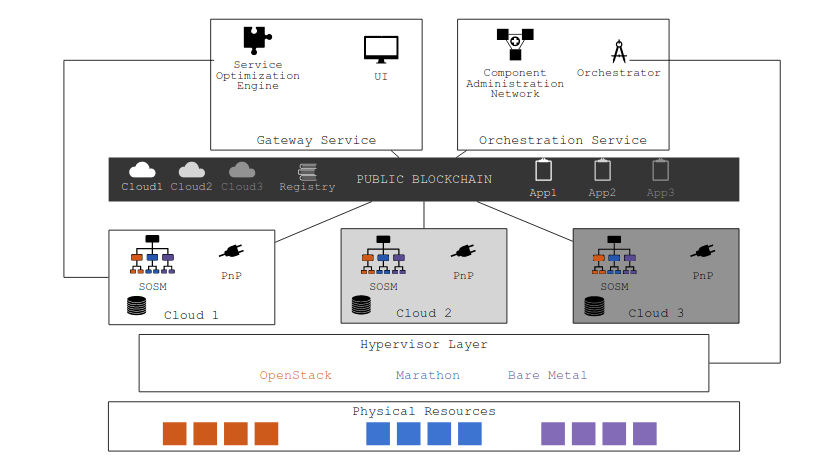
\includegraphics[width=1\linewidth]{figs/png/decentralizedcloudlightning}
  \caption{Augmented Decentralized CloudLightning Architecture}
  \label{fig:decent-cl}
\end{figure}


When a service fails, as mentioned, the Orchestrator will restart it
and the services depending on it will need to have the endpoints
updated to be able to keep communications.

There is a capability of decentralizing CloudLightning components,
which will be able to be discovered through \glspl{smart contract} on
a public blockchain.
%
This augmented architecture is presented in~\autoref{fig:decent-cl},
with the decentralized components:
\begin{itemize}
\item the registry contract keeps information on Cloud Providers,
  Services and Applications
\item the cloud contract keeps resources description (as well as their
  prices) and endpoints for the scheduler and Plug\&Play components
\item the application contract tracks deployment status and payments
\end{itemize}

Finally, the paper presents the Component Administration Networks
which make the link between Smart Contracts and Software components,
as well as giving monitoring and fault-tolerance capabilities to sets
of replicas.
%
This component is composed of three layers.
%
The first one is the underlying \acrshort{P2P} network of nodes that
collaborate and maintain the Ethereum blockchain.
%
The second layer manages the nodes thanks to a leader of the network,
that controls the transactions related to the component.
%
The third layer administer the components (such as (de)registration of
components, assign them some workload, etc.)


\subsubsection*{Comparison}

This approach is non-intrusive, using either VMs, containers or bare
metal, so it is also generic.

It does not follow the principle of local-first, as the services will
be separated depending on the best placement available, but those
services are allowed to collaborate through their configuration.

In case of a network partition, the services on the involved node will
probably be restarted elsewhere, but then the application on the
involved node will probably not be able to function as it would not
have all the services available.

Requests can be redirected to ``better'' computational resources
dynamically, but not on the user decision.
%
The users only define their requirements for the application.

This approach is fully decentralized and uses a blockchain to keep the
information on this decentralized approach.

% The authors use a blockchain and smart contracts for resource registration and assignment.


\subsubsection*{Conclusion}

In conclusion, this paper presents an enhance version of the
CloudLightning framework, to provide a decentralized orchestrator of
Cloud Services in the context of computing resources composed of home
computers or small-scale data centers.
%
The main goal of this paper is to pave the way for a decentralized
Cloud with individually owned resources serves as compute nodes, and
ways to deal with the payment of these resources.
%

The originality of this approach resides mainly on the use of a
blockchain and smart contracts to decentralize the control on the
orchestration.




\subsection{Liquid computing and Liqo~\cite{IRPCM22}}
\label{subsec:liqo}

Liqo is a solution to transparently manage different clusters in
Kubernetes, orchestrating them and allowing (computing) resource
sharing between those clusters.
%
The authors of the paper envision their approach, \emph{liquid
  computing}, as a continuum of resources and services to allow
transparent and infrastructure-agnostic deployment of applications.

For each workload, users can assign constraints such as geographical
locality, cost, capabilities, etc.
%
Their approach derives from a \acrshort{P2P} approach, with no centralized
control and no intrinsically privileged members.
%
Each actor (owner of a cluster) is the overall infrastructure keeps
the full control of their own infrastructure and decides how many
resources and services they share and with whom.
%
As in usual \acrshort{P2P} system, the topology is fluid and able to manage
dynamic changes, with frequent and sometimes unexpected connections
and disconnections.

It is built on different key concepts used for the liquid computing.
%
The first one is the discovery and peering functions. The peering in
their approach is a unidirectional resource and service consumption
relationship, which provides flexibility, but which can be combined to
support bidirectional peering.
%
Second, they distinguish nodes as local (attached to the consuming
cluster), virtual (abstracted and pooled resources) and big (for nodes
with much more capabilities than other average nodes), which allow
them to envision different types of clusters and a hierarchical
representation of the resources.
%
Third, to achieve robustness, tolerance to network disconnections and
scalability, they introduce the concept of resource reflection:
objects exist in their \emph{native} form in the local cluster and in
their \emph{shadow} form remotely.
%
Finally, the need for network, and storage and data continuum, where,
in the first one, the overlapping of different networks across the
cluster is a problem and should have a network fabric to handle
transparently this problem; and in the second one, the workload should
follow as much as possible its involved data.

Liqo itself is the project to enforce the liquid computing approach.
%
It extends -and is built upon- Kubernetes without any change in its
standard \acrshort{API}.

\subsubsection*{Comparison}

%
The approach is generic regarding the applications that will run in
the pods, but in itself, Liqo only works with Kubernetes solutions,
even though their key concepts could be applied to other orchestrator.
%

%
Each cluster works independently if need be, so it follows the rules
of local-first and collaborative-then, and thus a site can be used
during network partitions.

Liqo's approach needs some configurations to establish \acrshort{P2P},
but afterwards, the attribution of clusters is dynamic.
%
The location of execution of a request is chosen automatically per
scheduling, but \emph{intent-driven}, defined by users.
%, which means that the users can define a set of high-level policies
% to express associated constraints for the execution.

%
The goal of the approach is to offload pods on other sites by defining
unidirectional peering links, that can be combined to get a real
\acrshort{P2P} approach.

\subsubsection*{Conclusion}

The liquid computing concept and its associated project, Liqo aim at
envisioning a continuum of resources and services in a transparent and
infrastructure-agnostic manner.
%
The authors of the paper defined their vision, in which the main
characteristics are intent-driven definitions of the workloads,
decentralized architecture, multi-ownership and fluid topology.

From these principles, they deduce some pillars, key concepts, to allow
for the materialization of the liquid computing.
%
Finally, they present Liqo, their open-source project built on top of
Kubernetes to implement their vision through multi-cluster topologies.

Though this approach is really interesting in terms of our
requirements, the lack of user-defined requests at fined grain is
probably what is missing for the requirements.



\subsection{HYDRA: Decentralized Location-aware Orchestration of
  Containerized Applications~\cite{JS20}}
\label{subsec:JS20}

HYDRA~\cite{JS20} is a Proof of Concept (\acrshort{poc}) decentralized and
location-aware orchestrator that manages microservices in
containerized applications, written by Jimenez and Schelen.

In this paper, a focus is made on the location-aware version of the
orchestrator, even if it can run location-agnostic.
%
HYDRA builds a \acrshort{P2P} overlay network of nodes, where a node
is any hardware (virtualized or not) that can execute containerized
services, and thus a node is both orchestrator and (computing)
resource.
%
Four roles are available for the nodes:
\begin{itemize}
\item The entry role is temporary and corresponds to the role assumed
  when a node receive a request to deploy, remove or modify
  applications, where it needs to transfer this request to the
  appropriate nodes on the orchestrator network that will manage the
  request. The role is removed when the request has been served.
\item There are two controller roles, root and leaf, with the latter
  used only in location-aware control. The root controls the entire
  application, while the leaves manage only a set of services of the
  application.
\item The service host role is attributed to nodes who host and
  monitor services, and send heartbeats to the leader controller of
  those services for service liveness.
\end{itemize}

Depending on the number of required services, replicas of these
services, the need for scaling-out, and other considerations, the
number of service host nodes may change during the life-cycle of the
application.
%
These roles are not exclusive and a node can assume different roles
for different applications.

Users can deploy an application give its definition through a
\emph{recipe}, giving information on what and how to deploy, and how
it will be managed.
%
To deploy an application, the node in charge of deploying it launch
the search for viable nodes (in terms of resource availability with
the regards to the services requirements).
%
To find these nodes, the algorithm follows three properties:
\begin{itemize}
\item maximize the probability that the search will query different nodes
\item ensure that the load is spread across the HYDRA network evenly
\item leverage the information on the distance between nodes
\end{itemize}

Regarding the experiments, HYDRA is able to scale to at least 20 000
nodes, and support almost 30 000 applications running on 15 000 nodes.
%
The orchestrator nodes are able to work autonomously, and the location
awareness has almost no impact on the orchestrator performance.

\subsubsection*{Comparison}

Since it uses applications that run in containers, Hydra is non-intrusive
and generic to these existing Cloud applications.
%

The search for (computing) resources algorithm is randomized or use
new nodes as much as possible, so it is difficult to envision it is a
local-first approach.
%
Some services are deployed close to each other, but this is as local
as it gets.
%
On the other hand, it is a collaborative-then approach in the sense
that all resources can be used by any node.
%
The evaluation proves that the orchestrator itself still function in
case of network partitioning.
%

This approach can be considered dynamic because it requires a
configuration of the services, but then the requests are probably
routed depending on the application metadata, since some services are
replicated and so forth.
%
Because of that, the location is pre-defined from the users choice for
their applications, but afterwards, it is not chosen per-request.

The approach is designed to be fully decentralized, and all have nodes
can have the same privileges, even though they have different
privileges from the viewpoint of one application.


\subsubsection*{Conclusion}

HYDRA is a decentralized orchestrator for containerized microservices
based applications.
%
It allows for location-aware deployment and robust control of these
applications as well as management of heterogeneous Edge resources.
%
Finally, it provides resiliency of the deployed applications during
their life cycle.

This paper has many interesting approaches to solve problems that the
Edge can bring and follows a lot of our requirements.
%
Nonetheless, the location-awareness of the orchestrator does not allow
users to finely define the execution location of their request and it
lacks the requirement of local-first.


\section{Control planes and other managements}
\label{sec:other-management}

Some management tools do not fall into the orchestration category.
%
For example, \emph{control planes} are a layer in an application that will
manage higher functionalities such as monitoring, scaling, security,
configuration, etc. to make sure that the application runs properly
and as expected.
%
It is usually represented on top of the \emph{data plane}, which it controls,
as this one is the layer in charge of processing data requests, taking
orders from the control plane.

In this section, we will explore management solutions that can be seen
as these parts of the applications or just do not fit the
orchestration category.

\subsection{OneEdge: An Efficient Control Plane for Geo-Distributed
  Infrastructures~\cite{SGDR21}}
\label{subsec:SGDR21}

This paper from Saurez et al. presents a \emph{hybrid} control plane
for Edge infrastructures.
%
Like us, they consider infrastructures composed of different
micro-data centers, maintained by ISPs, with heterogeneous computation
resources.
%
They distinguish \emph{coordinated} applications which requires
collocation and coordination between different instances, such as
collaborative assisted driving and geo-distributed multiplayer games,
and \emph{standalone} applications which can work with a single
instance, such as virtual reality.
%
This approach is really interesting in the context of the Edge,
because it is easier to know where to put applications, depending on
these classes.
%
Some of the requirements they observed are also somehow close to ours:
\begin{description}
\item[Autonomous control] for latency-sensitive standalone
  applications, with single-site deployments
\item[Coordinated control] for coordinated applications, with
  multi-site deployments
\item[Spatial affinity] for applications location sensitivity
\item[End-to-end latency Service Level Objective] enforce the
  guarantees
\item[Dynamic resource allocation] for re-deployment in cases of
  mobility, failures, computing resource scarcity
\end{description}
Most of the differences have to do with the automated placement and
handling of users requests, and this is mainly were we have different
approaches.
%
In the context of the Edge (and more largely the Cloud), it is an
indubitably good idea and practice, but we chose to rely more on the
human intelligence and users and give them only information so they
can decide how to make their requests.

\subsubsection*{Comparison}

% no touching and genericity
OneEdge runs applications in containers and VMs, thus, without
changing their code. It is generic to existing Cloud
applications.

% Decentralization and \acrshort{P2P}
To coordinate applications instances, OneEdge has a centralized
controller to get a global view, but in order to keep autonomous,
rapid decisions without centralized coordination, an authoritative
state is kept on each site. The scheduling decisions are also left to
the Edge sites. Thus, most of the logic of the application is the same
everywhere, but not everything.


% LF CT
An effort has been made to decentralized the control plane as much as
possible, but keeping a central controller where decisions are made
(about placement and reallocation/migration through monitoring). The
collaborations between the sites are available for all types of
resources the control plane manages.

% NP
Most of the sites are autonomous, but for the centralized part, since
it is in the Cloud, fault tolerance is less important, but they ensure
it by having a secondary instance of the controller resubmitting the
requests (replicated on both instances) that have not be completed as
new requests. It is worth noting though, that the launch of
coordinated applications are forwarded to the central controller,
which is a problem in case of partitions.

% Dynamic OD
Users can request at any moment to launch an application, and these
requests are transferred to the closest site using a discovery
service. Thus, the control plane decide itself where a request will be
executed, but for each request, dynamically.


\subsubsection*{Conclusion}

OneEdge is a hybrid (in the sense of centralization) control plane
that allows some of the decision-making to be made autonomously on
Edge sites.
%
It presents an interesting approach to discriminate applications
between standalone and coordinated ones, which makes sense at the
Edge, because the needs are different.
%
To minimize deployment latency, standalone applications are scheduled
autonomously, while coordinated applications requires co-location and
thus, their deployment and scheduling is managed in a centralized
manner.
%
This hybrid approach of what can be done in a centralized manner or
not is a really interesting point that could be useful for other
approaches as it reduces the number of calls that will go to a
centralized \gls{dc}.
%
Nonetheless, it is not something I desired for my solution as I want a
decentralized and P2P approach.



\subsection{OpenYurt~\cite{openyurt}}
\label{subsec:oy}
OpenYurt is a platform extending Kubernetes to allow users to manage
large scale Edge computing workloads.
%
OpenYurt architecture is self-described like so:
\begin{quote}
  OpenYurt follows a classic cloud-edge architecture design. It uses a
  centralized Kubernetes control plane residing in the cloud site to
  manage multiple edge nodes residing in the edge sites. Each edge
  node has moderate compute resources available in order to run edge
  applications plus the required OpenYurt components. The edge nodes
  in a cluster can span multiple physical regions, which are referred
  to as Pools in OpenYurt.
\end{quote}

\autoref{fig:oy-arch} is the representation of OpenYurt architecture.
%
In this figure, the blue box represents the original Kubernetes
components, and the orange box the OpenYurt components.
%
This is a hierarchical approach in which Kubernetes \acrshort{API}
server is located in the Cloud, as well as OpenYurt Cloud node
management capabilities.
%
At the Edge part of the figure, the orange box represents what is
inside one node from any node pool on the right part.
%
Nodes at the Edge are composed of different Kubernetes
functionalities, such as Kubelet, KubeProxy, etc., and more
importantly of the pods themselves as well as OpenYurt Edge
functionalities.
%
For example, YurtHub serve as a sidecar to handle requests from
Kubernetes components on worker nodes and direct them to the
APIserver.
%
The connections from Edge nodes to the Cloud control plane is managed
by YurtTunnel (Server/Agent).


\begin{figure}[htbp]
  \centering  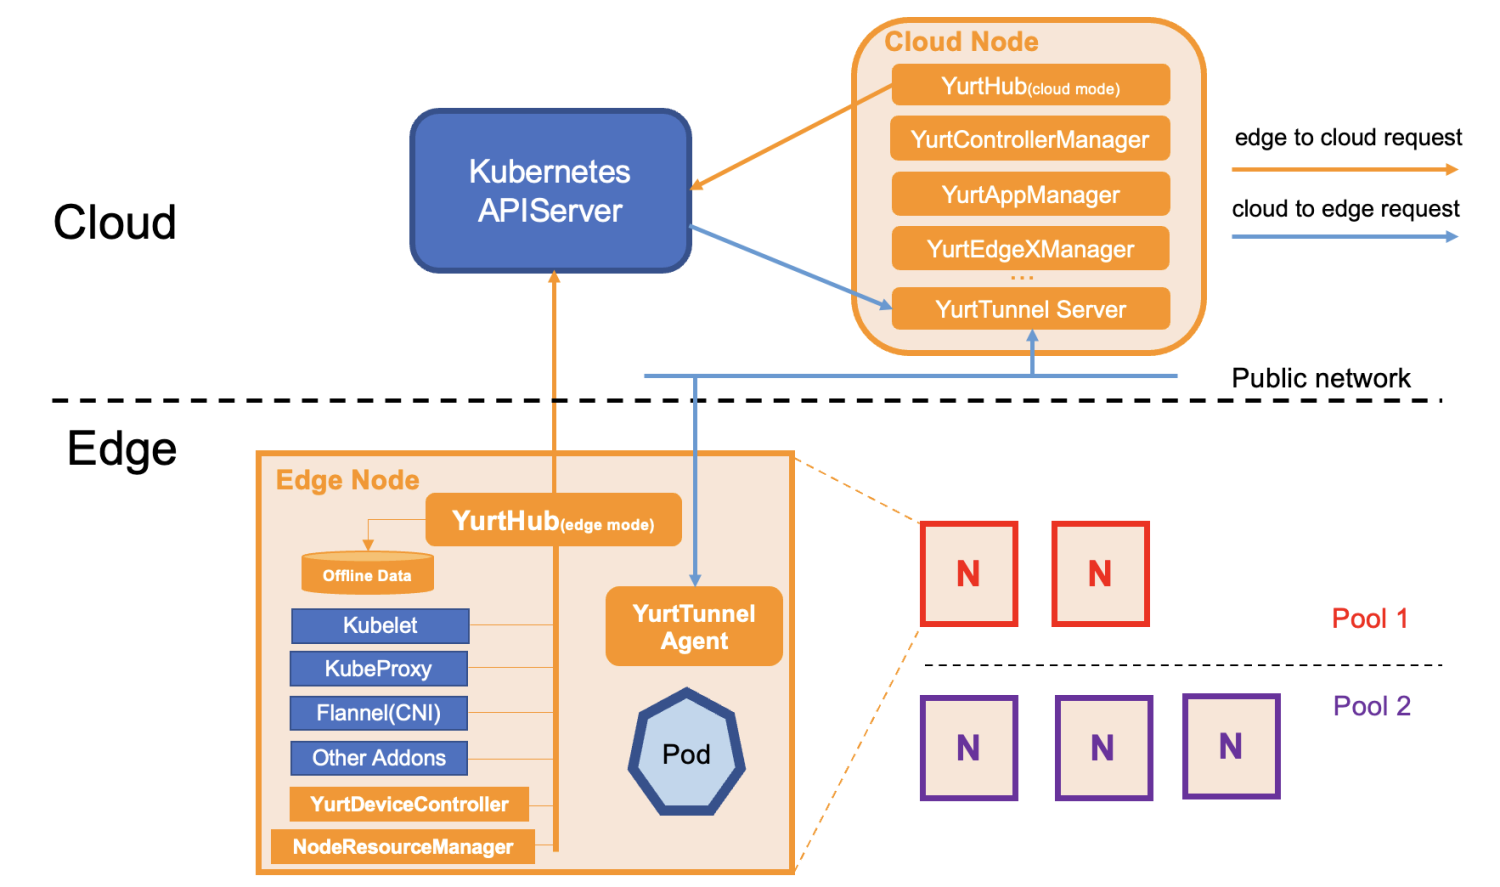
\includegraphics[width=.9\linewidth]{figs/png/openyurt-arch}
  \caption{OpenYurt architecture ( \href{https://github.com/openyurtio/openyurt}{Source: OpenYurt's Github}).}
  \label{fig:oy-arch}
\end{figure}

\subsubsection*{Comparison}

Using the original Kubernetes components, OpenYurt makes non-intrusive
enhancements, but the centralized control plane in the Cloud site
managing multiple Edge nodes makes it a not really \acrshort{P2P} approach.
%
It is generic to any application that can be run on Kubernetes.

%
Node autonomy is a functionality that allows Edge nodes to continue
running even though the Cloud-Edge link is severed, but it is only
available through configuration.
%
Moreover, node autonomy only means that users can manipulate existing
resources and not create new ones, so its partition tolerance is not
complete.

The collaboration are available for every resources managed by
Kubernetes.

%
It is worth mentioning that \emph{service topology} allows users to
decide to use in general the endpoints from the same node, or from the
same nodepool, so the general location execution of the request (by
general location policies) is decided globally by the users, and then
the application chose the exact location.

As it as a centralized control plane and a hierarchical architecture,
it is not decentralized and is not a \acrshort{P2P} system.

\subsubsection*{Conclusion}

OpenYurt is a self-described \emph{platform} that extends Kubernetes
to deliver a non-intrusive approach which can allow network partition
to some extent (\ie whatever does not need the control plane).
%
Regarding our requirements, it answers not entirely the local-first
and collaborative-then principles, as well as the network partition in
node autonomy mode.
%
Moreover, it lacks a decentralized approach and the ability for users
to make finely defined requests.



\subsection{Re-designing Cloud Platforms for Massive Scale using \acrshort{P2P}
  Architecture~\cite{SYHJ17}}
\label{subsec:SYHJ17}

In\cite{SYHJ17} (and~\cite{Han17}), Soares et al. present a way to use
\os on a large scale, using \acrshort{P2P} architecture.
%
Though it is not designed specifically for the Edge, scaling is the
first step towards a solution for the Edge, and the \acrshort{P2P} approach
checks some of our requirements.
%
They briefly introduce the concepts that were introduced in \os to
manage large scale deployments, such as Regions to manage the locality
of resources, or Availability zones which allows to logically
partition compute, storage or network resources, and finally Cells,
which allows to shard several compute resources into cells, and then
be dispatched in different locations.
%
But all these solutions had to be \emph{added} into \os code, and thus
are available whether you need them or not.

They follow three design principles:
\begin{itemize}
\item avoid centralized components as much as possible, for
  scalability and robustness purposes.
\item avoid as much as possible changes in the original code so it is
  easily adopted and can be more generic.
\item externalize problems to an existing outside system as much as
  possible to simplify the solution and minimize the efforts.
\end{itemize}

%
They deploy an entire instance of the Cloud management software on
every sites, calling the instance a \gls{cloudlet}.

%
On each site, they put their agent which can send a request to the
local \os or forward it to another site.
%
This agent implements a service proxy on each \os service.
%
Each proxy around a service expose the same \acrshort{API} as the
service they encapsulate, as well as request forwarding and
translation logic.
%
This follows the broker based collaboration presented
in~\autoref{sec:why-no}.
%
Each agent is also composed of an \emph{overlay management} which
allow the different agents to discover each other and identify which
agent sent a particular request.
%
Each agent has a \emph{state management} to allow them to keep
information about users and resources they own.
%
Finally, an interface allows the agents to communicate with each other
(Agent-to-Agent communication).

Each agent is responsible to handle every requests that come from any
user mapped with it.
%
This mapping is statically created when a user's tenant is created.
%
Through state management, each agent tracks the resources allocated to
a tenant, which is required to find resources that are not stored
locally but on other sites.
%
They keep they internal ID of the created resources and map them to
the cloudlet where the resource has been provisioned.
%
To improve robustness, this state information can be replicated on
several agents, but their implementation uses a simple database.

%
As a \acrshort{P2P} system, each site maintains a list of their
neighbors, where a transitive closure of the graph representing the
neighbor relationships returns all sites in the system.
%
More simply put, with every lists of the neighbors of every sites,
there is a complete view on the entire system.

Regarding specific services, they use the federated identity for
authentication and authorization, which is a service-to-service
functionality offered by \os.
%
For the image service, the image is found thanks to the mapping of
ID/site presented above.
%
For the scheduling/placement of VMs, they chose to balance the memory
load on all sites.
%
Finally, for the network, they do not use a specific approach but
mention it is a problem that is being addressed.
%
They mention the Tricircle approach~\cite{tricircle}, but since this
article is a bit dated, I would also like to mention this
approach~\cite{ELNC20}, which was one of the first steps for a part of
our own solution.


\subsubsection*{Comparison}

One of their design principles is to avoid touching the code as much
as possible, and in the paper, there is actually no mention of having
to change the code.
%
In their principles, they also mention that the external approach is
to make it generic, but no further fact is given about this, so we
consider it to be designed specifically for \os, even though it
probably can be adapted for this purpose.
%
In any case, since this approach manages a infrastructure manager, it
is generic to any application that could be run in an \os VM.

They operate an entire instance of \os on each cloudlet, so it works
perfectly locally on a standalone way.
%
It is collaborative through federation of some of the services and
through the agent for the rest.

The \acrshort{P2P} approach combined with the fact that there is an instance on
each site makes it tolerant to network partition.

The placement of the tenant is determined statically at its creation,
but otherwise, other requests are dynamic, following the list of
neighbors the agents know.
%
If some of the resource are treated locally as possible; the VMs,
which are somehow the principal resource of \os are automatically
placed, so we cannot really say it is per user request.

The approach is entirely decentralized and without hierarchical
management, designed as a \acrshort{P2P} system.



\subsubsection*{Conclusion}

This paper presents an approach to decentralize \os in a
non-intrusive and \acrshort{P2P} manner, with autonomous instances.

In this approach, images from Glance (the image service) are shared
across different sites.
%
They use internal IDs from their agent to keep tracks of these
resources shared on different sites with a mapping to IDs created by
\os to find the resources locally.
%
This is something really useful for our local-first and
collaborative-then principles and has actually been used in our
solution.

%
Since our initial focus was on \os, this paper was obviously
important in our early decision making, and especially before we
decided we needed a more generic and user-centric approach.



\section{Conclusion on managing applications on Edge infrastructure}
\label{sec:soa-em-conclusion}

To ease the reading of the table, we add the following reminder, for orchestration:
\begin{description}
\item [\cite{Spataru20}] Decentralized and Fault Tolerant Cloud Service Orchestration (\autoref{subsec:spataru20})
\item [\cite{IRPCM22}] Liquid computing and Liqo (\autoref{subsec:liqo})
\item [\cite{JS20}] HYDRA: Decentralized Location-aware Orchestration of Containerized Applications (\autoref{subsec:JS20})
\end{description}
And for control planes and other managements:
\begin{description}
\item [\cite{SGDR21}] OneEdge (\autoref{subsec:SGDR21})
\item [\cite{openyurt}] OpenYurt (\autoref{subsec:oy})
\item [\cite{SYHJ17}] Re-designing Cloud Platforms for Massive Scale using P2P Architecture (\autoref{subsec:SYHJ17})
\end{description}

\begin{table}[htbp]
  \centering
  \footnotesize\setlength{\tabcolsep}{4pt}
\begin{tabular}{|c|c|c|c|c|c|c|c|c|c|}
\hline
 & NI & generic & LF & CT & NP & dynamic & on-demand &  decentralized & P2P\\
\hline
  \cite{Spataru20} & \cloud \cloud \cloud  & \cloud \cloud \cloud  & - & \cloud \cloud \cloud  & \cloud  & \cloud \cloud \cloud  & \cloud  & \cloud \cloud \cloud  & \cloud \cloud \cloud \\
  \cite{IRPCM22} & \cloud \cloud \cloud  & \cloud \cloud  & \cloud \cloud \cloud  & \cloud \cloud \cloud  & \cloud \cloud \cloud  & \cloud \cloud  & \cloud \cloud  & \cloud \cloud \cloud  & \cloud \cloud \\
  \cite{JS20} & \cloud \cloud \cloud  & \cloud \cloud  & \cloud  & \cloud \cloud \cloud  & \cloud \cloud \cloud  & \cloud \cloud  & \cloud  & \cloud \cloud \cloud  & \cloud \cloud \cloud \\
  \hline
  \cite{SGDR21} & \cloud \cloud \cloud  & \cloud \cloud \cloud  & \cloud \cloud  & \cloud \cloud \cloud  & \cloud  & \cloud \cloud \cloud  & \cloud  & \cloud \cloud  & \cloud \cloud \\
  \cite{openyurt} & \cloud \cloud \cloud  & \cloud \cloud  & \cloud \cloud (1) & \cloud \cloud \cloud  & \cloud(1) & \cloud \cloud  & \cloud  & \cloud  & \cloud \\
  \cite{SYHJ17} & \cloud \cloud \cloud  & \cloud \cloud  & \cloud \cloud \cloud  & \cloud \cloud  & \cloud \cloud \cloud  & \cloud \cloud  & \cloud \cloud  & \cloud \cloud \cloud  & \cloud \cloud \cloud \\
  \hline
  \end{tabular}
  \caption{Comparison points on Edge infrastructure management.
    (1) Only available when activating node autonomy\protect\footnotemark.}
  \label{tab:soa-eim}
\end{table}


\footnotetext{\url{https://openyurt.io/docs/next/user-manuals/autonomy/node-autonomy}}

\autoref{tab:soa-eim} represents the comparison of the approaches to
orchestrate and manage Edge infrastructure to deploy applications.

The first part (the three first lines) are defined as orchestrators,
while the others are respectively identified as only a control plane,
a platform and an architecture for an existing management platform.

Whatever the name, they all can be used deploy workflow and
applications, via virtualization or containerization.

In terms of existing Cloud applications that are brought to the Edge,
\os is used in one of these approaches~\cite{SYHJ17}, while Kubernetes
is used in two of those approaches (\cite{IRPCM22, openyurt} and other
aforementioned approaches from the Orchestration introduction.
%
\cite{Spataru20} uses an existing project, CloudLightning as a base on
which to build upon.

The main requirement lacking in those approaches are the user-centric
decisions, but otherwise, some applications make solid candidate
regarding our base requirements introduced
in~\autoref{sec:principles}, such as~\cite{IRPCM22, openyurt},
though~\cite{openyurt} only offers tolerance to disconnections as a
\emph{degraded} mode.


Since none of the approaches corresponds entirely to my requirements,
we will now take interest in a way that could help to manage the
different instances of the application we want at the Edge, and
especially the collaborations between them.




\section{A service mesh at the Edge?}
\label{chap:soa-SM}

% Linkerd (one of the most used service mesh) defines a service mesh
% as~\cite{linkerd-sm}:
% \begin{quote}
%   A service mesh like Linkerd is a tool for adding observability,
%   security, and reliability features to “cloud native” applications by
%   transparently inserting this functionality at the platform layer
%   rather than the application layer. The service mesh is rapidly
%   becoming a standard part of the cloud native stack, especially for
%   Kubernetes adopters.
% \end{quote}

William Morgan from Buoyant Inc. (Buoyant created Linkerd, one of the
most used service mesh) defined services meshes as~\cite{LLGZG19}(© 2011 IEEE):

\begin{quote}
A service mesh is a dedicated infrastructure layer for handling
service-to-service communication. It’s responsible for the reliable
delivery of requests through the complex topology of services that
comprise a modern, cloud native application. In practice, the service
mesh is typically implemented as an array of lightweight network
proxies that are deployed alongside application code, without the
application needing to be aware.
\end{quote}

In practice, a service mesh helps with the separation of the tasks of
development from the operations.
%
The developers can focus on the business logic and code, and operators
on deploying the application, keeping it running, etc., as put by
William Morgan: [the service mesh is] ``deployed alongside application
code, without the application needing to be aware''.
%
Actually, RedHat specified that~\cite{redhat-sm}:
\begin{quote}
  Without a service mesh, each microservice needs to be coded with
  logic to govern service-to-service communication, which means
  developers are less focused on business goals.
\end{quote}
%
In this sense, a service mesh could help with the service
collaborations discussed in~\autoref{sec:c-to-e-solutions}.


It usually consists in a scalable set of proxies deployed with the
application~\cite{linkerd-sm}, as specified by William Morgan in the quote above.
%
These proxies, composing the \emph{data plane}, manage the
communications between the micro-services, passing them through the
\emph{control plane} to execute whichever functionalities the service
mesh provides.

\autoref{fig:sm-arch} presents an abstracted service mesh
architecture.
%
The control plane and the data plane are represented
separated.
%
Each service is deployed alongside a proxy as a sidecar,
but the proxy could also be represented as the capsule around the
service, because it intercepts incoming and outgoing communications to
transfer them to the control plane.
%
These proxies thus serve both as proxies and as reverse
proxies~\cite{rproxy}.
%
In the control plane, there are different components achieving the
functionalities of the service mesh, such as monitoring, service
discovery (to build a registry of services), etc.
%
Also, since it is an abstract representation, there can be any number
of services or components, which is shown as the dots on the right
part of the figure.

\begin{figure}[htbp]
  \centering  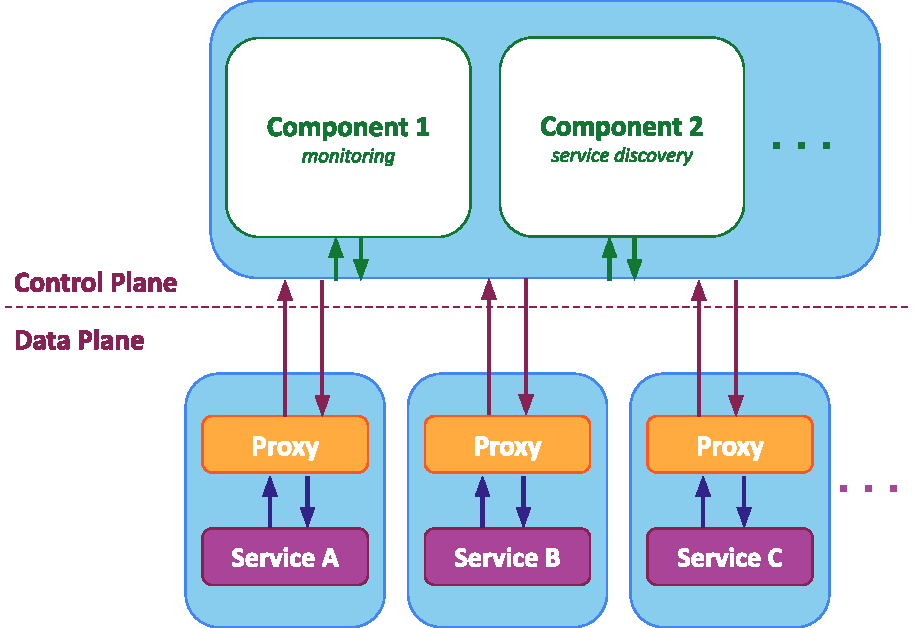
\includegraphics[width=0.75\linewidth]{figs/pdf/service-mesh}
  \caption{Architecture of a typical service mesh, inspired from \cite{SMmanifesto}}
  \label{fig:sm-arch}
\end{figure}


Though service meshes were not created in the first place for the
Edge, they are a very important software architectural framework for
Edge computing, because they could bring functionalities such as
service discovery, load-balancing, resiliency, scalability,
low-latency offloads and privacy~\cite{GRRL+21, LLGZG19}.



\subsection{Istio~\cite{SS20}}
\label{sec:soa-istio}

Istio is an open source service mesh that uses
Envoy\footnote{\url{https://www.envoyproxy.io/} - Accessed:
  2022-09-20} as the proxy.
%
Envoy is a proxy often used as a
dataplane\footnote{\url{https://servicemesh.es/} - Accessed:
  2022-09-20} and is deployed as a sidecar along each service.
%
Envoy has a L3, L4 and L7 filter layer, which allows to filter and
route \acrshort{TCP}/\acrshort{UDP}, \acrshort{TLS} (see \gls{tcp},
\gls{udp}, \gls{tls} for definitions), HTTP(/2) and \acrshort{gRPC}
requests, with much more functionality on the last two.


Istio provides traffic management through Envoy and service-level
properties (timeouts, retries, etc.) configurations, through the Istio
Pilot agent running in the sidecar or the gateway container.
%
The control plane also provides observability through the tracking of
requests, which allows for example to track dependencies between
services, how they interact between each other, and also metrics to
control the system.
%
Historically, the control plane was composed of four components,
namely Pilot (service discovery), Galley (configuration), Citadel
(certificate generation), and Mixer (extensibility).
%
But since in 2020, Istio has been delivered as a signal binary,
Istiod, to simplify the process of deployment and because a lot of the
benefits of micro-services did not make sense in Istio context.

\autoref{fig:istio} represents a multi-cluster version of Istio: the
mesh covers three different clusters (in orange) on two different
networks (in black).
%
Traffic goes through Envoy (the pink hexagon), whether it is inside a
cluster (green arrows), or between clusters (dotted blue arrows).
%
If the West-North cluster goes down, the West-South can take the load
temporary.
%
Those two cluster communicate with each other thanks to being in the
same network.
%
In such a configuration, all services are shared, and if the share the
same namespace, they will be considered as a single combined service.
% https://github.com/istio/istio.io
%https://github.com/istio/istio.io/blob/master/content/en/docs/ops/deployment/deployment-models/multi-cluster.svg
\begin{figure}[htbp]
  \centering  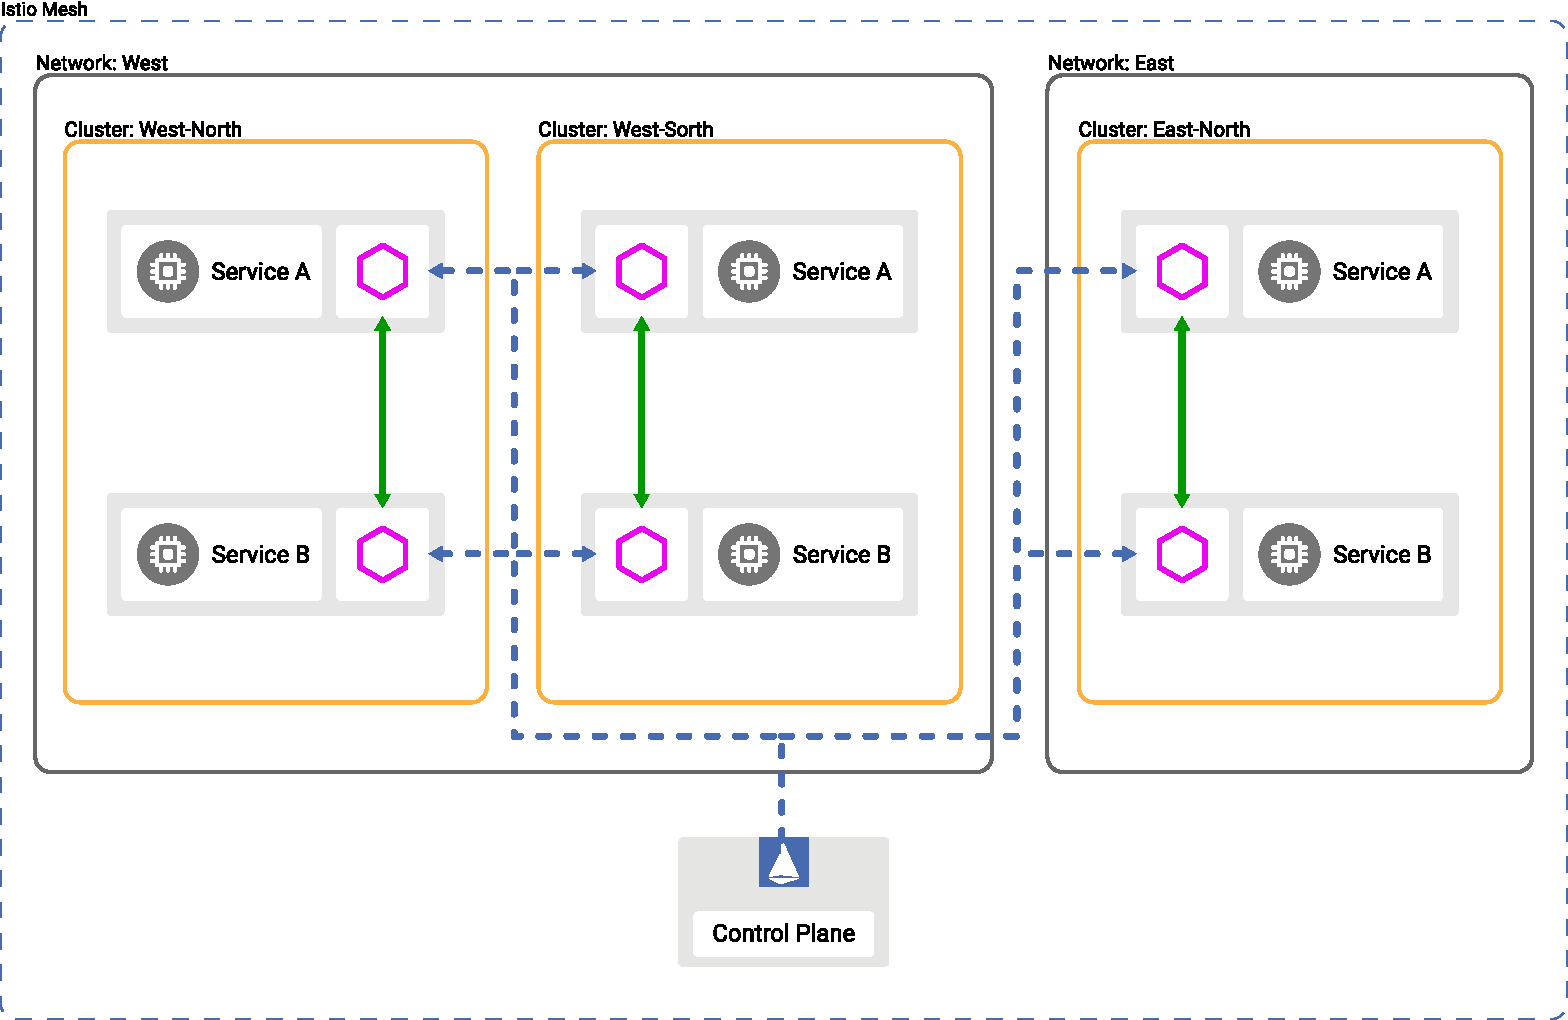
\includegraphics[width=0.75\linewidth]{figs/pdf/istio-multi-cluster}
  \caption{Multiple clusters on Istio}
  \label{fig:istio}
\end{figure}


\subsubsection*{Comparison}

It is mostly generic to applications that can be used in
Kubernetes\footnote{\url{https://istio.io/latest/docs/ops/deployment/requirements/}
  - Accessed: 2022-09-20}.
%
Since it extends Kubernetes, there is no changing the code for many
applications, however, some might require some changes, depending if
the application requirements are met or not yet.
%
This requirements \emph{for some applications} have given Istio a
three/two clouds for non-intrusion, for fairness.
%

Since multi-cluster is only supported with a central control plane, we
do not consider that it can survive a network partition.
%
Of course, though, if one site is cut off from the rest, users can
still use another site.
%
In mesh
federation\footnote{\url{https://istio.io/latest/docs/ops/deployment/deployment-models/\#multiple-meshes}
  - Accessed: 2022-09-20}, it might be possible, but even with the
Google
demo\footnote{\url{https://github.com/GoogleCloudPlatform/istio-samples/tree/master/multicluster-gke/dual-control-plane}
  - Accessed: 2022-09-20}, the information given on the functionality
is not sufficient to determine this (especially because it seems to
mostly allow service spreading across potentially different sites, but
at minimum different meshes).

The configuration of the deployment is prepared statically, and can be
updated depending on the users needs.

The location of execution of requests is determined through Envoy
load-balancing, so it is automatically chosen.

Since Istio has been designed for the Cloud, its control plane is
centralized, and thus, most of the functionalities are executed there.
%
Finally, there is no real point in talking about Istio \acrshort{P2P}
capabilities, except for this
example\footnote{\url{https://banzaicloud.com/blog/istio-multi-mesh/}
  - Accessed: 2022-09-20}, where they achieved a multi-mesh,
multi-cluster which can be considered as a \acrshort{P2P} version of Istio, so it
is technically possible, though not designed for this.
%

\subsubsection*{Conclusion}

Istio is a service-mesh using Envoy as a sidecar proxy for every
services.
%
Some efforts have already been made to allow multi-cluster in Istio,
though it is still not designed to be entirely autonomous and
decentralized as the control plane is centralized (at best one per
region).
%
Thus, it is going in a really good direction for us, with some
possibilities to make a P2P version, it is still lacking user chosen
locations for executing requests, as it is done automatically.



\subsection{Linkerd~\cite{linkerd}}
\label{sec:soa-linkerd}

Linkerd is another service mesh, which was the first called like that.
%

Linkerd, like Istio, allows to filter and route \acrshort{TCP},
\acrshort{TLS}, HTTP(/2) and \acrshort{gRPC} requests, with much more
functionality on the last two.


Linkerd2 uses
Linkerd2-Proxy\footnote{\url{https://github.com/linkerd/linkerd2-proxy}
  - Accessed: 2022-09-20}, an ``ultralight micro-proxy'' tailored for
their needs to make Linkerd smaller and simpler.
%
Linkerd developers decided that Envoy had too much
functionalities which made it inappropriate for a sidecar use.
%
Whether it is for the complexity, the resource consumption, or the
danger of having such a complex proxy introducing security issues in
its code, they preferred a lightweight approach that work perfectly
for their use case.
%
The downside is that it is not recommended to use Envoy as a proxy and
Linkerd2-proxy would not be usable by another service
mesh\footnote{\url{https://linkerd.io/2020/12/03/why-linkerd-doesnt-use-envoy/}
  - Accessed: 2022-09-21}.

\autoref{fig:linkerd} shows an overview on how Linkerd deal with the
Multiple Cluster functionality.
%
Clusters (here, west and east) communicates with each other through a
Multi-Cluster gateway.
%
This gateway is then responsible to route a request from a Service
from the other cluster to the involved Service in its own cluster.
% https://github.com/linkerd/website/blob/main/linkerd.io/static/images/multicluster/feature-overview.svg
% https://linkerd.io/2.12/features/multicluster/
\begin{figure}[htbp]
  \centering  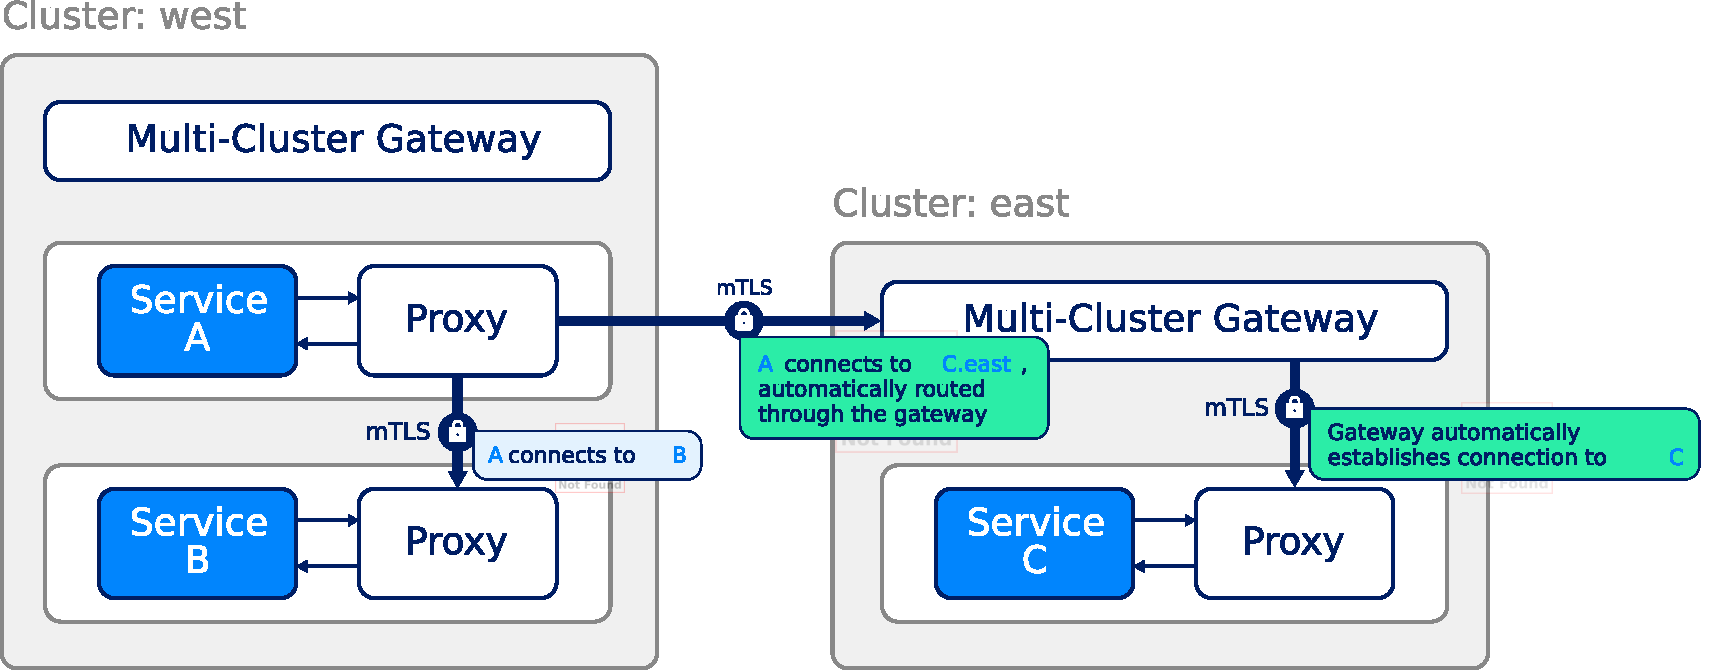
\includegraphics[width=0.75\linewidth]{figs/pdf/linkerd-multi-cluster}
  \caption{Multiple clusters on Linkerd}
  \label{fig:linkerd}
\end{figure}

\subsubsection*{Comparison}

Linkerd, as for most service meshes, does not require any change in
the business code of the underlying applications, though it is also
specific to Kubernetes, because it only consider resources managed by
Kubernetes (with mesh expansion on the
roadmap\footnote{\url{https://github.com/linkerd/linkerd2/blob/main/ROADMAP.md}
  - Accessed: 2022-09-21}).

It is design to work locally first since it is supposed to be running
in the Cloud, but in multi-cluster, it is possible to get resources
from other services.


The recommendations on how to make an architecture for multi-cluster
Kubernetes give these architectures with Linkerd a solid chance of
surviving network
partitions\footnote{\url{https://linkerd.io/2020/02/17/architecting-for-multicluster-kubernetes/}
  - Accessed: 2022-09-21}.
%
They recommend to maintain independent states between clusters and
manage updates via replications so updates are only where required.
%
They also advise to keep the control planes independent separate,
which further makes the system more tolerant to network partitions.
%
When the control plane is down, though, the proxies will use the
information they already have and fall back to \gls{Domainns} (\acrshort{DNS}) if a
request is supposed to be routed to a service they do not know.
%
But this implies that any proxy deployed when the control plane is
down will need to timeout all new requests until the control plane is
up
again\footnote{\url{https://linkerd.io/faq/\#what-happens-to-linkerd-s-proxies-if-the-control-plane-is-down}
  - Accessed: 2022-09-21}.
%
In conclusion, Linkerd in multi-cluster mode is tolerant to network
partitions, but not entirely.

Regarding dynamicity, Linkerd uses an algorithm called Exponentially
Weighted Moving Average (EWMA) to automatically route requests to the
fastest
endpoints\footnote{\url{https://linkerd.io/2.12/features/load-balancing/}
  - Accessed: 2022-09-21}.
%
The execution location of a request is chosen for the user, in part
through traffic split.

As for Istio, we cannot consider this application of the \acrshort{P2P} point,
since it has not really been designed to work with several instances
of the application.

\subsubsection*{Conclusion}

Linkerd is a service mesh that relies on a homemade, lightweight and
less generic proxy than Envoy, called Linkerd2-Proxy.
%
It also supports a multi-cluster architecture if need be, through
gateways on each cluster that redirects the request they receive
locally to the required service.


\subsection{Conclusion on service meshes}
\label{sec:soa-sm-conclusion}

We studied two different service meshes which mostly have the same
functionalities and goals, except that Linkerd seems to be more
focused on being lightweight.
%
In the appendix (\autoref{chap:first-approach}), we
will also talk a bit about Consul, which has been considered as a
solution for us for a time.

\begin{table}[htbp]
  \centering
  \footnotesize\setlength{\tabcolsep}{4pt}
\begin{tabular}{|c|c|c|c|c|c|c|c|c|c|}
\hline
 & NI & generic & LF & CT & NP & dynamic & on-demand & decentralized & P2P\\
\hline
Istio & \cloud \cloud \cloud /\cloud \cloud  & \cloud \cloud  & \cloud \cloud \cloud  & \cloud \cloud  & \cloud  & \cloud \cloud  & \cloud  & \cloud  & -\\
Linkerd & \cloud \cloud \cloud  & \cloud \cloud  & \cloud \cloud \cloud  & \cloud \cloud  & \cloud \cloud  & \cloud \cloud  & \cloud  & \cloud \cloud  & -\\
  \hline
  \end{tabular}
  \caption{Comparison points on service meshes.}
  \label{tab:soa-sm}
\end{table}

Overall, service meshes could be a good solution to our main research
question of putting Cloud applications to the Edge if they were
designed for the Edge, to be more collaborative, more decentralized,
and more generic.
%
It is especially true since they are doing more and more efforts to
support multi-clustering (both propose versions of this functionality,
with different levels of support) and more application managers.

It is also noteworthy that despite some efforts, service meshes are
pretty demanding and impact the performance of small devices, so there
is a lack in service meshes that would be able to be used at the
Edge~\cite{GRRL+21}.
%
A lightweight version that checks our requirements might be the
solution to our research questions, and especially this one: ``since
service meshes are designed to manage the communications between
services of an application outside of its business code, can it be a
solution to using Cloud applications on Edge infrastructures without
changing their code?''.


As we did not find an approach that fits entirely the requirements, we
will now consider techniques to make applications at the Edge in order
to learn if some ideas could help us in building a generic solution on
the main question raised in this manuscript.



\chapter{How to make Edge applications natively}
\label{chap:soa-dev-edge-app}

Though we think it is better to not reinvent the wheel, and so use as
much as possible Cloud applications directly on the Edge, it is still
possible to develop an Edge application from scratch.
%
First, it makes sense of course simply for new applications that will
be developed with the Edge in mind.
%
Second, some frameworks might have been developed to do so, in case
some of them might automatize the process of pushing an application to
the Edge, which could work on an existing Cloud application.
%
Third, some approaches might give guidelines on how to properly
develop an application for the Edge~\cite{RYHL19}, which is of interest even to know
how to push an existing Cloud application to the Edge.

\section{Towards Scalable Edge-Native Applications~\cite{WFGI+19}}
\label{sec:WFGI+19}

\cite{WFGI+19} from Wang et al. presents an approach to ``edgify'' an
application, \ie the Gabriel platform~\cite{HCHR+14}, that was
designed for a single user.
%
Though this approach is mainly about multi-tenancy, because Gabriel
was already an application to offload the functionalities of IoT to
Fog/Edge, it gives requirements for the Edge.
%

Since the authors are changing Gabriel to be more scalable, they talk
about the enhance version as "Scalable Gabriel", while the other is
"Original Gabriel".
%
In this paper, they refer to a three tier architecture of the Cloud
computing.
%
The Tier-3 would be the Edge, composed of IoT and mobile devices, and
where data are pre-processed in the Gabriel front-end (\eg compression
and encoding).
%
The Tier-2 would correspond to the Fog (what we refer to as the Edge),
composed of cloudlets, small \acrshort{DC}s, etc., and where the
Gabriel back-end and its different modules treat the data from the
Tier-3.
%
The Tier-1 would be the Cloud itself, with further and bigger
\acrshort{DC}s, with more compute power, energy usage and elasticity.

The original Gabriel was built for a single user, \ie only one sensor
interacting with one cloudlet (1:1), and they want to allow several
devices to interact with the same cloudlet (n:1).

Several applications run on the original Gabriel Platform, but the
authors focus on Wearable Cognitive Assistance (WCA, running typically
on glasses for Augmented Reality in their cases) applications because
they deem that these applications present three crucial
characteristics for Edge computing:
\begin{itemize}
\item they transmit large volumes of (video) data from the device to
  the cloudlet (Tier-3 to Tier-2, or in our case, we would say from
  the devices to the Edge).
\item they have strict latency requirements
\item they impose high computing demands on the cloudlet, especially
  in the GPUs.
\end{itemize}
Regarding the last characteristic, the workflow of these applications
in the cloudlet is composed of two phases.
%
The first phase treat the images to extract an abstract, symbolic
representation of the state of the task, while the second phase, far
less compute intensive, operates on this symbolic representation,
implementing the logic of the task.

To tackle the scalability problems, they first reduce the load going
through the wireless network and to the cloudlet through adaptation
(\emph{Workload reduction}); the second is about a better scheduling
of cloudlet resources to minimize queuing and impacts of potential
overloads (\emph{cloudlet resource allocation}).
%
Both those approaches are tested afterwards.

To adapt the original Gabriel to these points, they leverage the WCA
applications characteristics.
%
The first is the \emph{human-centric timing}, which corresponds to the
fact that the applications have active phases, where they need to
sample and process video frames to give instructions to the users,
which will perform these instructions in the passive phase of the
applications.
%
In this passive phase, the sampling and processing of video frames to
determine if the user has soon finished the instructions, which would
considerably reduce the load.

The second is \emph{event-centric redundancy}, where they detect
redundant frames that do not provide new information to reduce the use
of the wireless bandwidth and the cloudlet cycles on frames.

The third is \emph{inherent multi-fidelity}, in which they leverage
the fact that some of the processing algorithms can trade-off fidelity
and computation.
%
When a cloudlet becomes overloaded by multiple
applications, it is possible to act on this trade-off to ensure the
applications functionalities.

Finally, they give a taxonomy of relevant adaptations depending on the
characteristics of the applications. These adaptation techniques are
presented in ~\autoref{table:WFGI+19}.

\begin{table}[h!]
  \begin{center}
    \begin{scriptsize}
      \begin{tabular}{|c|p{4.5cm}|p{5.5cm}|p{4cm}|}
        \hline
        & & & \\
        & \textbf{Question}      & \textbf{Example}   & \textbf{Load-reduction Technique}    \\
        & & & \\
        \hline
        1         & How often are instructions given, compared to task duration?    & Instructions for each step in IKEA lamp assembly are rare compared to the total task time, e.g., 6 instructions over a 10 minute task.    & Enable adaptive sampling based on active and passive phases.    \\
        \hline
        2 & Is intermittent processing of input frames sufficient for giving instructions? & Recognizing a face in any one frame is sufficient for whispering the person’s name. & Select and process key frames.   \\
        \hline
        3 & Will a user wait for system responses before proceeding? & A first-time user of a medical device will pause until an instruction is received. & Select and process key frames. \\
        \hline
        4 & Does the user have a pre-defined workspace in the scene? & Lego pieces are assembled on the Lego board. Information outside the board can be safely ignored. & Focus processing attention on the region of interest.\\
        \hline
        5 & Does the vision processing involve identifying and locating objects? & Identifying a toy lettuce for a toy sandwich. & Use tracking as cheap approximation for detection.\\
        \hline
        6 & Are the vision processing algorithms insensitive to image resolution? & Many image  classification DNNs limit  resolutions to the size of their input layers. & Downscale sampled frames  on  device before transmission.\\
        \hline
        7 & Can the vision processing algorithm trade off accuracy and computation? & In image classification, MobileNet is computationally cheaper than ResNet, but less accurate. & Change computation fidelity based on resource utilization.\\
        \hline
        8 & Can IMUs be used to identify the start and end of user activities? & User’s head movements are of significantly higher magnitude when searching for a Lego block. & Enable  IMU-based  frame suppression.\\
        \hline
        9 & Is the Tier-3 device powerful enough to run parts of the processing pipeline? & A Jetson TX2 can run MobileNet-based image recognition in real-time. & Partition the vision pipeline between Tier-3 and Tier-2.\\

        \hline
      \end{tabular}

      \centering
      \caption{Application characteristics and corresponding
        applicable techniques to reduce load (Source: Wang et
        al.~\cite{WFGI+19}).}
    \label{table:WFGI+19}
  \end{scriptsize}
  \end{center}
\end{table}

Then, they proceed in testing these techniques for workload reduction,
as mentioned above.
%
From these evaluations, the authors are able to conclude that
Edge-native applications should be written in very different way from
Cloud-native applications to be scalable.


\subsubsection*{Comparison}

Since this paper is about specific use-cases (WCA applications) that
requires some computing locally and most of it in what we call Edge
computing, the question of collaboration is difficult, since
collaborations is only vertical (from one Tier to another) and not
horizontal (between multiple sites of the same Tier).
%

The approach is about modifying an existing application (original
Gabriel), but the overall logic did not change.
%
It is generic for any (WCA) application that can run on the Gabriel
platform only, but the adaptations are much wider and could be used
both to adapt a Cloud application or to build and Edge application.

%
Monitoring of the resources is done on both tiers of the involved
architecture (Tier-3 and Tier-2), but some are monitored at Tier-3,
others at Tier-2.
%
As said before, the collaboration is only vertical and most resources
are not managed locally, so it is only some part of the computation
that is available locally \textbf{and} it only a subset of resources
is used in collaboration.

%
Once again, because of the verticality, network partition is tricky.
%
If we consider network partition in the same tier, it will not be a
problem, since there is no collaboration inside.
%
But, in the context of WCA applications, on a wireless network, there
is a even larger chance of a partition between any of the devices and
the cloudlet, and thus, any offload computation could not be
done. Thus, only one cloud is awarded, for the case of partition in
the same tier.

The authors do not debate the n:n relationship between devices and
cloudlets, so there is no real dynamic choice of the location of
execution of requests, and the same can be said for the user ability
of choosing the location.

% Since WCA applications are designed to make computation further away
% from the devices, it is difficult to call them ``Cloud
% applications''. And if we consider using the Gabriel platform, it is
% the same problem; as well as the fact that they changed it.

The cloudlet is the actual only place of execution of the tasks, no
mention of a re-balancing to other cloudlets, so the approach is
hierarchical and centralized.

Because the Tier-3 Gabriel front-end is not the same as its back-end
Tier-2 counterpart, and most of the workload is done in the cloudlet,
we cannot say this approach is a \acrshort{P2P} system.

\subsubsection*{Conclusion}

In conclusion, this approach is a redesigned version of Gabriel, a
platform to allow a single wearable device process data in a cloudlet,
to allow the cloudlet to manage several devices.
%
By degrading the quality of service when it is possible and not
required, the cloudlet is able to withstand a much higher load and
number of connected devices than previously, as well as the wireless
network load is decreased.
%
They defined a taxonomy of applications and a set of rules to apply to
allow a smarter processing of the data recorded by edge devices, which
could be reusable to adapt a Cloud application for the Edge as well as
to develop a new Edge-native application from scratch.
%
This approach, by only considering only vertical relations
(edge-devices to cloudlet), is not using the entire capabilities of
the Edge and is designed specifically for small edge devices that need
to offload almost all their workloads to the Edge servers/Fog.

This solution is pretty interesting for the ideas on how to adapt an
application for the Edge, even though it is mainly aimed at WCA
applications because they leverage some of their unique
characteristics.
%
One conclusion in this paper I found really interesting is they
consider that Edge-native applications should be written very
differently from Cloud-native ones to be scalable.
%
It is probably true for applications running on the Edge devices, but
it would be interesting to test on Edge servers, since it would be
that we cannot have a non-intrusive approach.


\section{Highly-Available and Consistent Group Collaboration at the
  Edge with Colony~\cite{TSS21}}
\label{sec:TSS21}

Colony~\cite{TSS21, Toumlilt21} by Toumlilt et al. is composed of a
middleware and a database to address the lack of approaches for
collaborative applications at the Edge.
%


\begin{figure}[htbp]
  \centering  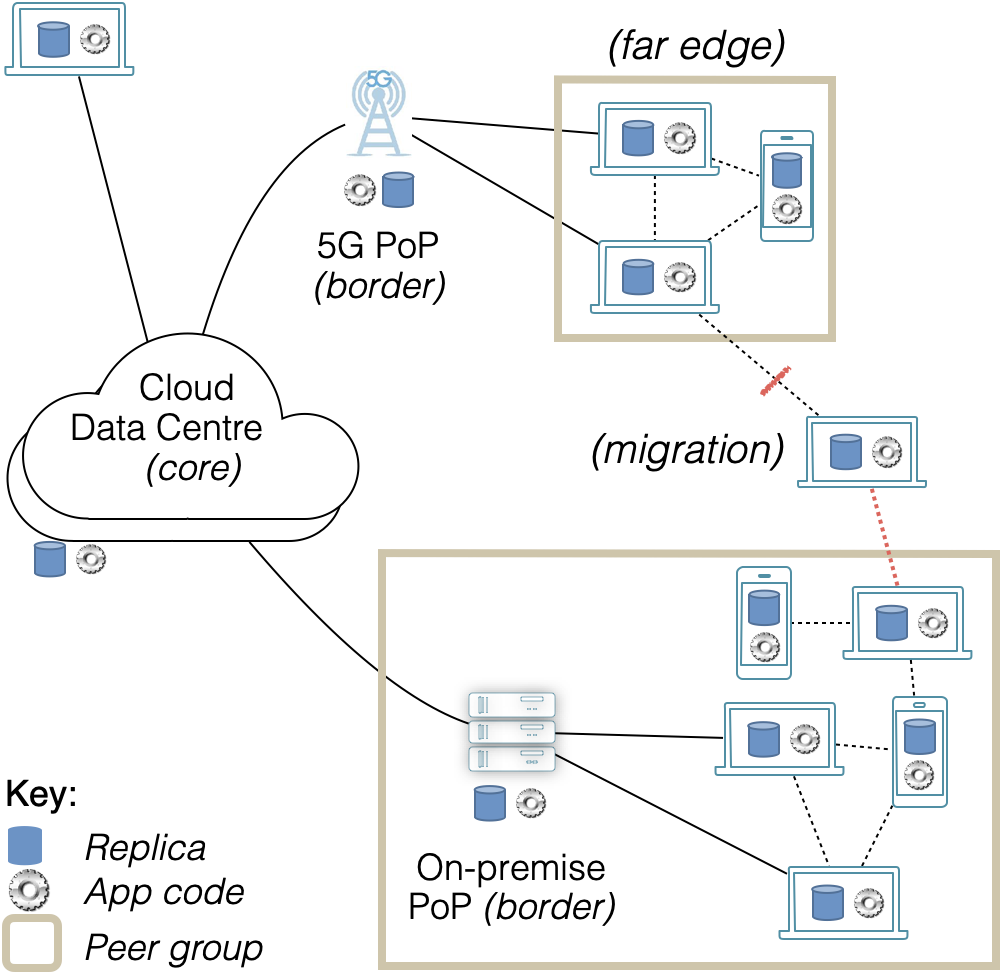
\includegraphics[width=.6\linewidth]{figs/png/colony-topology}
  \caption{An example of a Colony topology (Source:~\cite{Toumlilt21}).}
  \label{fig:colony}
\end{figure}

The database responds to the need of Edge-to-Cloud continuum and is
designed for collaborative applications.
%
In a typical usage, presented in~\autoref{fig:colony}, the Cloud core
is composed of a small number of \acrshort{DC}s, and the Edge nodes
are grouped by proximity, connecting either to the core \acrshort{DC}s
or to a PoP server at the border of the group.
%
Due to mobility, a node can migrate from one group to another.


The focus of this work is consistency in the Edge with a local-first
approach.
%
As such, they enforce a hybrid approach for consistency: globally, the
model follows a Transactional Causal Plus Consistency (TCC+)
introduced in the paper; in the data centers, the consistency provided
is Snapshot Isolation (SI), as the servers are connected through
high-quality networks; finally, in the local groups, they also enforce
SI, but the system needs to be able to work disconnected to keep them
available and without losing the overall TCC+ guarantees, using
EPaxos.

The TCC+ model guarantees causal consistency~\cite{ANBKH95},
rollback-freedom (no rollbacks after a value has been read), strong
convergence (any two nodes observing the same set of updates read the
same value), atomicity, snapshot.
%
It extends the TCC model~\cite{ZPDBVS15} with the strong convergence
and rollback-freedom


\subsubsection*{Comparison}

The Colony middleware is designed to provide a simple \acrshort{API}
to develop and deploy collaborative applications at the Edge.
%
This means that some effort is made to help developers to make their
applications collaborative at the Edge, but it is thus a very
intrusive method to follow the necessary data types and \acrshort{API}.
%
%It also means that it is not made to use existing Cloud applications.
%
This approach is generic to any type of collaborative applications for
the Edge.

The local-first principle is one of the focus of the approach, and it
is enforced by replications and caches.
%
There are collaborations (in our sense) between the nodes in the same
group especially when needed, on any types of resources.

The application is supposed to be able to work offline with the entire
system and design, so in effect, it supports network partitions: ``the
application can read and write data, even when disconnected from any
remote server''.

The required information are transmitted to required nodes
dynamically, even in case of mobility.
%
The location of execution of requests is mainly local, and on the
peers of the collaborative applications.
%
Data is replicated and cached depending on the edge client
\emph{interest}.

The approach is hierarchical, as some transactions are run only in
the core Cloud, such as analytics or large queries.
%
The core also manages the authentication of nodes via the session
manager, but it is only for the current implementation.


\subsubsection*{Conclusion}

In conclusion, Colony is an approach to design collaborative
applications for the Edge, guaranteeing the highest consistencies
possible for the availability of the resources in the context of the
Edge.
%
To do so, it follows a hybrid approach in consistency, using TCC+ in
the global cases ans Snapshot Isolation in the peer, Edge groups.
%
It allows migration of nodes between groups for mobility and ensures
fault-tolerance and scalability by having the groups replicated
roots in the Cloud.
%

Overall, it is a really interesting approach to design collaborative
applications for the Edge, which is robust, mostly decentralized,
generic and follows the base principles of local-first and
collaborative-then.

As a final note, this approach uses a shared database approach, which
we did not want to use for reasons presented
in~\autoref{ssec:issue-db}, but makes sense if properly used for a
new application, developed from scratch.

% The trade-off is that, during some failures, liveness cannot be
% ensured. A client cannot make progress in two cases: if it requires
% data that cannot be retrieved; or if it runs out of storage. Further-
% more, there are corner cases (described later) where a client commits
% updates, but they cannot become visible. The above situations are
% temporary, and last only until the problem is repaired.





\section{Conclusion on ways to make an application at the Edge}
\label{sec:soa-edge-conclusion}


To ease the reading of the table, we add the following reminder:
\begin{description}
\item [\cite{WFGI+19}] Towards Scalable Edge-Native Applications (\autoref{sec:WFGI+19})
\item [\cite{TSS21}] Highly-Available and Consistent Group Collaboration at the Edge with Colony (\autoref{sec:TSS21})
\end{description}


\begin{table}[htbp]
  \centering
  \footnotesize\setlength{\tabcolsep}{4pt}
    \begin{tabular}{|c|c|c|c|c|c|c|c|c|c|}
      \hline
       & NI & generic & LF & CT & NP & dynamic & on-demand &  decentralized & P2P\\
      \hline
      \cite{WFGI+19} & \cloud & \cloud \cloud  & \cloud  & \cloud \cloud  & \cloud  & - & - & \cloud  & \cloud \\
      \cite{TSS21} & \cloud & \cloud \cloud \cloud  & \cloud \cloud \cloud  & \cloud \cloud \cloud  & \cloud \cloud \cloud  & \cloud \cloud \cloud  & \cloud \cloud  & \cloud \cloud  & \cloud \cloud \\
      \hline
  \end{tabular}
  \caption{Comparison points on making applications at the Edge.}
  \label{tab:soa-edge}
\end{table}

\autoref{tab:soa-edge} sums up the comparison on the approaches to
make applications at the Edge.

Both approaches are pretty different and do not focus on the same
requirements.

%
In~\cite{WFGI+19}, the focus is about making intelligent choices (both
in design and by the use of adaptive algorithms) to lower the load
when possible and allow several applications to run on the same node.
%
Thus, it also gives clues on how to adapt an existing Cloud
application for the Edge, but keeping only its functionality logic and
changing entirely the way it is used.

%
In~\cite{TSS21}, the authors focus on bringing consistency,
scalability and offline mode to collaborative applications at the
Edge.
%
Moreover, the approach follows the local-first principle, same as us,
which makes it a particularly strong candidate to answer our
requirements, but it lacks the decentralized, \acrshort{P2P} system
that leaves the users the ability to choose the execution location of
their requests.


Both answer parts of the puzzle of building an Edge-native
applications.




\chapter{Comparison and conclusion on the State of the Art}
\label{chap:soa-conclusion}

\section{Comparison }
\label{sec:soa-comparison}


To ease the reading of the table, we add the following reminder, for
approaches that can't be in a single word:
\begin{description}
\item [\cite{Spataru20}] Decentralized and Fault Tolerant Cloud
  Service Orchestration (\autoref{subsec:spataru20} - Decentralized
  CloudLightning)
\item [\cite{SYHJ17}] Re-designing Cloud Platforms for Massive Scale
  Using a P2P Architecture (\autoref{subsec:SYHJ17} - P2P OpenStack)
\item [\cite{WFGI+19}] Towards Scalable Edge-Native Applications
  (\autoref{sec:WFGI+19} - Scalable Gabriel)
\end{description}

\begin{table}[htbp]
  \centering
  \footnotesize\setlength{\tabcolsep}{2pt}
\begin{tabular}{|c|c|c|c|c|c|c|c|c|c|}
\hline
Approach & NI & generic & LF & CT & NP & dynamic & on-demand & decentralized & P2P\\
\hline
  \cite{Spataru20} & \cloud \cloud \cloud  & \cloud \cloud \cloud  & - & \cloud \cloud \cloud  & \cloud  & \cloud \cloud \cloud  & \cloud  & \cloud \cloud \cloud  & \cloud \cloud \cloud \\
  Liqo~\cite{IRPCM22} & \cloud \cloud \cloud  & \cloud \cloud  & \cloud \cloud \cloud  & \cloud \cloud \cloud  & \cloud \cloud \cloud  & \cloud \cloud  & \cloud \cloud  & \cloud \cloud \cloud  & \cloud \cloud \\
  HYDRA~\cite{JS20} & \cloud \cloud \cloud  & \cloud \cloud  & \cloud  & \cloud \cloud \cloud  & \cloud \cloud \cloud  & \cloud \cloud  & \cloud  & \cloud \cloud \cloud  & \cloud \cloud \cloud \\
  OneEdge~\cite{SGDR21} & \cloud \cloud \cloud  & \cloud \cloud \cloud  & \cloud \cloud  & \cloud \cloud \cloud  & \cloud  & \cloud \cloud \cloud  & \cloud  & \cloud \cloud  & \cloud \cloud \\
  OpenYurt\cite{openyurt} & \cloud \cloud \cloud  & \cloud \cloud  & \cloud \cloud & \cloud \cloud \cloud  & \cloud & \cloud \cloud  & \cloud  & \cloud  & \cloud \\
  \cite{SYHJ17} & \cloud \cloud \cloud  & \cloud \cloud  & \cloud \cloud \cloud  & \cloud \cloud  & \cloud \cloud \cloud  & \cloud \cloud  & \cloud \cloud  & \cloud \cloud \cloud  & \cloud \cloud \cloud \\
  \hline
  Istio~\cite{SS20} & \cloud \cloud \cloud  & \cloud \cloud  & \cloud \cloud \cloud  & \cloud \cloud  & \cloud  & \cloud \cloud  & \cloud  & \cloud  & -\\
  Linkerd\cite{linkerd} & \cloud \cloud \cloud  & \cloud \cloud  & \cloud \cloud \cloud  & \cloud \cloud  & \cloud \cloud  & \cloud \cloud  & \cloud  & \cloud \cloud  & -\\
  \hline
  \cite{WFGI+19} & \cloud  & \cloud \cloud  & \cloud  & \cloud \cloud  & \cloud  & - & - & \cloud  & \cloud \\
  Colony~\cite{TSS21} & \cloud  & \cloud \cloud \cloud  & \cloud \cloud \cloud  & \cloud \cloud \cloud  & \cloud \cloud \cloud  & \cloud \cloud \cloud  & \cloud \cloud  & \cloud \cloud  & \cloud \cloud \\
  \hline
  \end{tabular}
  \caption{Comparison points on the overall state of the art.}
  \label{tab:soa-comp}
\end{table}

\autoref{tab:soa-comp} represents the overall comparison according to
the different categories.

There is no solution that fits entirely the requirements,
but there are some that fit perfectly or almost our principles of
local-first and
collaborative-then~\cite{TSS21,IRPCM22,SGDR21,openyurt,SYHJ17}.

A lot of the different solutions considered overall had a
non-generic approach, except for how to build a Edge-native
application, of course.
% all of the solutions are non-intrusive because
% it was crucial for us.


A requirement that is also mostly overlooked is the resilience to
network partitions, with four approaches that do not have a way to
cope with it, even when we do not count service meshes that were
designed for the Cloud (and thus need it less).
%
In the context of the Edge, it is unreasonable to neglect site
autonomy when disconnections are the norm rather than the exception.


In terms of putting Cloud applications to the Edge, the solutions
studied leverage a distributed database in two
cases~\cite{Spataru20,TSS21}, while others use some sort of brokering
or service-to-service~\cite{SYHJ17, WFGI+19} without the
location-aware aspects to make it less intrusive.
%
And interestingly, the non-intrusive requirement is the one that is
mostly observed, except for solutions to build applications for the
Edge, which makes sense for Edge-native applications.

As for the genericity, it is mainly provided by allowing to deploy
containerized applications~\cite{IRPCM22, JS20, openyurt, linkerd,
  SS20} or applications in containers, VMs, and sometimes more (like
bare metal)~\cite{Spataru20, SGDR21}.

As mentioned in the more specific comparisons, the user-centric to
have on-demand, dynamically managed requests is what is mostly lacking
from the approaches, though dynamicity is considered
at request level in three solutions.
%
This is the point that definitely needs to be taken into account for
our solution, if we want to allow users to define where they want
their requests to be executed.


% If we exclude the service meshes that were not designed specifically
% for the Edge, the consideration of the network partition is stunningly
% not enough considered, since disconnections at the Edge must be
% considered the norm rather than the exception.


\section{Conclusion }
\label{sec:soa-conclusion}

In this part, we have seen different solutions to allow applications
running at the Edge.

%
One of the goals was to find original (and different from one another,
except for the service meshes), generic and/or usable approaches that
have not been studied already by members of our project, such as in
Manaouil et al.\cite{ML20}.


%
This State of the Art does not cover specific subjects in the
deployment and life cycle of applications services, such as algorithms
in charge of discovery, monitoring, load-balancing or placement, but
rather tried to focus on solutions that fit at least some of them, to
have ideas on how it is dealt with.
%
Of course, still in the context of having applications at the
Edge.
%
It is also sidelining approaches to manage the physical, hardware Edge
infrastructure that study how to put computing devices in the
infrastructure because it was out of scope, and we considered that
we had the infrastructure ready to use.
%

%
Some of the solutions presented here are really good answers to the
Edge challenges in their own way, and only fail our own requirements.

%
The hierarchical approaches, for example, create Single Point of
Failure (\acrshort{spof}) and bottlenecks, and thus cannot be
envisioned as solutions unless they have mechanisms to avoid those
problems (replication~\cite{TSS21}, temporary autonomy~\cite{SS20},
etc.).
%
The lack of tolerance to network partitions/disconnections is also a
problem in the context of the Edge, as mentioned before.
%
Finally, the lack of dynamic and on-demand, only when required
collaborations, with most of the workload executed as locally as
possible, is what drove the approach we built and will now detail.

What can be taken away from this State of the Art, regarding the
requirements:
\textbf{
\begin{itemize}
\item While a lot of approaches are collaborative, not enough respect
  the local-first principle or the tolerance to network partitions,
  which is a problem in the context of the Edge.
\item Approaches that are generic concentrates mostly on deploying
  containerized applications, especially with Kubernetes, without
  considering the collaborations that could be done between the
  deployed application.
\item Solutions often consider dynamicity of the requests, which is a
  good thing in a highly dynamic context, but they do not consider
  enough the will of the users by allowing the execution location to
  be chosen on-demand by the users.
\end{itemize}
}
None of the solutions answered to all the requirements, but the
service mesh approaches could be leveraged to make a service dedicated
to managing the geo-distribution in a decentralized and P2P manner,
outside of the business code, similar to the multi-cluster approach of
Linkerd.
%
This point of view will be more detailed and explained in the next
part, with our own solution.

% The requirements on dynamicity and per-demand user requests are
% important to us, but the user-centric requirement is definitely not
% the priority in the solutions studied.
%






% \chapter{Using Cloud Applications at the Edge}
% \label{chap:soa-c-to-e}

% \todoref{cf sources in comments}
% % https://itnext.io/superedge-openyurt-extending-native-kubernetes-to-edge-cc59094f92c
% % https://medium.com/volterra-io/control-plane-for-distributed-kubernetes-paas-e20a82acd6d3
% % https://landscape.cncf.io/?license=open-source&grouping=no
% % https://liqo.io/
% % https://krossboard.app/docs/01_overview-concepts-features/

% \todono{titles}
% \section{Using databases}
% \label{sec:soa-dbs}

% \section{Using broker}
% \label{sec:soa-broker}

% \section{Using service-to-service}
% \label{sec:soa-s-to-s}

% %\section{Using containers}

% \chapter{Using service meshes at the Edge}
% \label{chap:soa-SM}


% \subsection{Istio}
